The instances come from the project's own generator (\texttt{sample\_instance}, seed 901) with $N = 3$ drones, so that the MILP, the heuristic and the learned policy all see the same geometry. Gurobi 13.0.2 ran with six threads on a machine that was concurrently training the reinforcement-learning agent. The lattice uses $\kappa = 10$ simulator steps per period and $h = 98.2$\,m.

\begin{table}[h]
\centering
\caption{Model size and search outcome. Makespan is in simulator steps (seconds). ``best'' is the best incumbent over the runs listed; the spread shows how much the incumbent varies between identical runs with different solver seeds.}
\label{tab:milp}
\begin{tabular}{rrrrrrrr}
\toprule
$M$ & $|N|$ & $\bar{T}$ & binaries & runs & best & spread & bound \\
\midrule
4 & 99 & 18 & 5913 & 5/5 & 140 & 140--170 & 81 \\
6 & 98 & 23 & 7539 & 1/2 & 180 & --- & 100 \\
10 & 107 & 30 & 10941 & 0/2 & none & --- & --- \\
\bottomrule
\end{tabular}
\end{table}

\begin{table}[h]
\centering
\caption{The best MILP plan replayed in the simulator, against the geometric relay rule with deadlock escape on the same instance. ``cut'' counts the drone-steps in which the simulator's connectivity projection shortened a commanded displacement, the price of sampling connectivity only at period boundaries.}
\label{tab:replay}
\begin{tabular}{rrrrrr}
\toprule
$M$ & MILP & replayed & cut steps & rule & $C_{\mathrm{LB}}$ \\
\midrule
4 & 140 & 138 & 22 & 145 & 50 \\
6 & 180 & 176 & 59 & 185 & 53 \\
10 & none & --- & --- & 244 & 57 \\
\bottomrule
\end{tabular}
\end{table}

Two facts stand out. The incumbent is unstable: 5 runs of the same $M = 4$ model with different solver seeds returned makespans from 140 to 170\,s. And the primal side degrades sharply with the number of destinations: at $M = 4$, 5 of 5 runs returned a feasible plan, at $M = 6$, 1 of 2 runs returned a feasible plan, at $M = 10$, 0 of 2 runs returned a feasible plan. The model is a reference for the smallest instances only. Where it does return a plan, the plan is good: replayed in the simulator it beats the geometric rule with deadlock escape (138 against 145\,s at $M = 4$; 176 against 185\,s at $M = 6$), and it never loses connectivity. The cut-step counts in Table~\ref{tab:replay} are the price of sampling connectivity at period boundaries: the simulator had to shorten that many commanded displacements, without ever disconnecting a drone.

\begin{figure}[h]
\centering
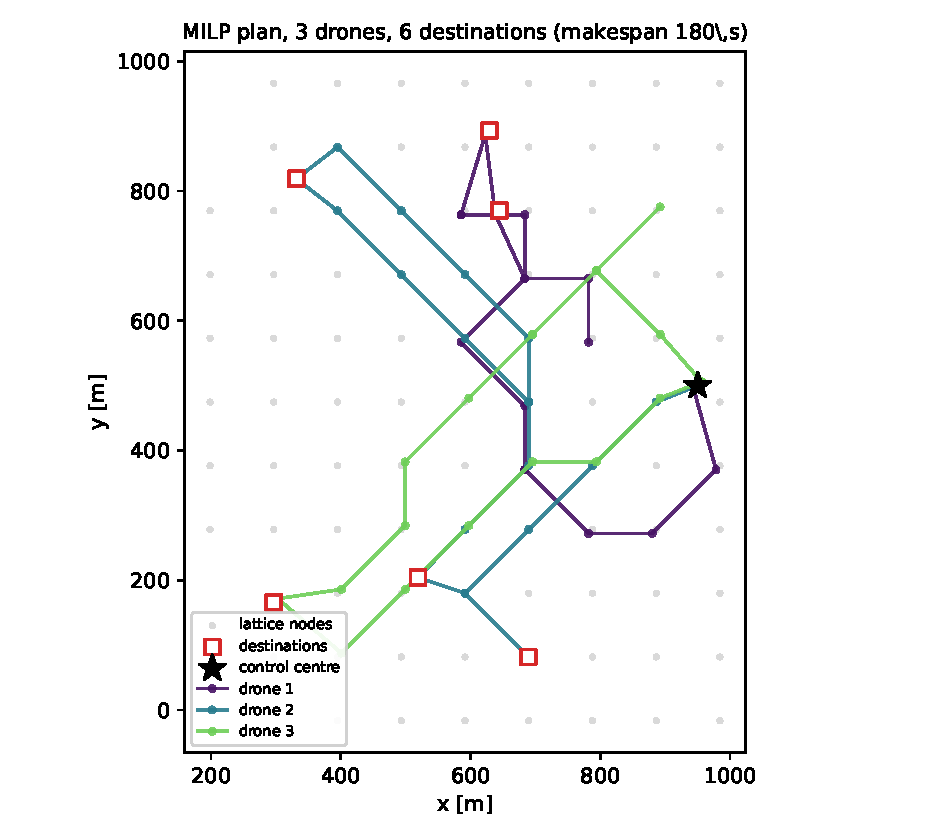
\includegraphics[width=0.70\textwidth]{../../figures/milp_plan_v5_26_09_21_03.pdf}
\caption{Lattice, destinations and optimal trajectories for the largest instance the model could solve. Trajectories are offset by a few metres per drone so that shared nodes stay visible.}
\label{fig:plan}
\end{figure}
